\documentclass{ltxdoc}
\usepackage{tikz}
\usepackage{xkeyval}
\usepackage{huaslogo}
\usetikzlibrary{positioning}
\usepackage{xcolor,colortbl}
\usepackage{verbatim}   
\usepackage{caption}
\usepackage{subcaption}
\usepackage{titlesec}
\usepackage{float}
\usepackage{pgf}

\setlength{\parskip}{12 pt}
\titlespacing*{\section}
{0pt}{0ex}{0ex}
\titlespacing*{\subsection}
{0pt}{1ex}{-1ex}
\titlespacing*{\subsubsection}
{0pt}{1ex}{-1ex}

\newcommand{\boxwidth}{0.45\textwidth}
\newcommand{\boxheight}{0.15\textwidth}


\title{Huaslogo, v. 1.0\\
\large Logos for the Hanze university of Applied Sciences Groningen}

\author{Arjan Kloekhorst\\
\href{mailto:a.kloekhorst@pl.hanze.nkl}{a.kloekhorst@pl.hanze.nl}}

\date{January 2023}

\begin{document}
\setlength{\parindent}{0cm}

\maketitle

{\parskip=0pt \tableofcontents}
\newpage

\section{Introduction}
The package \verb|huaslogo| containes the dutch and english logos for the Hanze university of Applied Science Groningen, including the logo for "share your talent. move the world.". This latex package is based on the  \verb|thuaslogos| from Jesse op den Brouw. The packages \verb|xkeyval|, \verb|xcolor| and of course \verb|tikz| need to be loaded for proper working of the package.  
\par
The package can be loaded with:
\par
\verb|\usepackage{huaslogo}|
\par
\section{Version}
The latest version can be found at:
\par
\url{https://github.com/ArJKloek/huaslogo.git}
\section{Used colors}
The Hanze unviversity of Applied Science Groningen has three main colors defined for the logo: 
\par 

\begin{table}[h]
    \centering
    \begin{tabular}{m{0.25\textwidth}m{0.25\textwidth}m{0.25\textwidth}}
     \begin{tikzpicture}
         \node[rectangle ,minimum height = 0.15\textwidth, minimum width = 0.15\textwidth, fill = huasorange](orange) at (0,0){};
     \end{tikzpicture}    &  
     
\begin{tikzpicture}
         \node[rectangle ,minimum height = 0.15\textwidth, minimum width = 0.15\textwidth, fill = black](black) at (0,0){};
     \end{tikzpicture}  & 
     \begin{tikzpicture}
         \node[rectangle ,minimum height = 0.15\textwidth, minimum width = 0.15\textwidth, draw, color = gray, fill = white](black) at (0,0){};
     \end{tikzpicture}\\
      Orange   & Black & White \\ \\ 
      PMS: Pantone 158 & PMS: Black &  \\
      RGB: 238/127/0 & RGB: 0/0/0 & RGB: 255/255/255
    \end{tabular}
\end{table}
White and black are already standard colors in \LaTeX\ therfore only
one color needed to be defined in the package as \verb|huasorange|: 
\par
\verb|\definecolor{huasorange}{RGB}{238,127,0}| \\
\clearpage
\section{Macros}
The following macros are availible with the additional options:
\par
\cmd{\huaslogo}\oarg{scale, rotate, opacity, logocolor, textcolor, EN, onlylogo, }
\par
\cmd{\huasSYTMTW}\oarg{scale, rotate, opacity, SMcolor, YTTWcolor, square}
\par
The \cmd{\huaslogo} macro with no added options will give the following logo: \\
\begin{figure}[h]
\centering
\huaslogo
\caption*{\cmd{\huaslogo} with no options entered}
\end{figure}
\\
The \cmd{\huasSYTMTW} macro with no added options will give the following logo: \\
\begin{figure}[h]
\centering
\huasSYTMTW
\caption*{\cmd{\huasSYTMTW} with no options entered}
\end{figure}
\par
\clearpage
\section{Keys}

The following arguments for \verb|\huaslogo| and \verb|huasSYTMTW| can be given in the style as \verb|\huaslogo[key = value]|. The following keys are defined:
\begin{itemize}
    \item [\verb|scale|:] This key sizes the logo by the use of the \verb|\scalebox| macro. The default behavior of this key is 1.
    \item [\verb|rotate|:] Here the angle $(0 - 360)$ of the logo can be changed by the use of the \verb|\rotatebox| macro. The default behavior of this key is 0.
    \item [\verb|opacity|:] Here the opacity of the logo can be changed $(1 - 0)$ this if done by the use of \verb|\pgfsetfillopacity|. The default behavior of this key is 1.
    \item [\verb|logocolor|:] Here the color of the logo of \verb|\huaslogo| can be changed. The default color is given as huasorange, due to the use of \verb|xcolor| other standard colors of latex like \verb|red| or \verb|gray| can also be used. Mixing of colors like \verb|red!10| is also possible. User declared colors by using \verb|\definecolor|\ can also be used.   
    \item [\verb|textcolor|:] Here the color of the text of the \verb|\huaslogo| can be changed. The default color is given as black, also here the colors can be changed as explained in \verb|logocolor|.
    \item [\verb|SMcolor|:] Here the color of the \textbf{share move} part of the \verb|huasSYTMTW| can be changed. The default color is given as huasorange. Also here the colors can be changed as explained in \verb|logocolor|. 
    \item [\verb|YTTWcolor|:] Here the color of the \textbf{your talent. the world.} part of the \verb|huasSYTMTW| can be changed. The default color is given as black. Also here the colors can be changed as explained in \verb|logocolor|. 
\end{itemize}
The following keys are boolean and can be used as \verb|\huaslogo[key]|. The use of the \verb|key| without the need for the addition of \verb|= true| is possible due to the use of the \verb|boolkey| option in the \verb|xkeyval| package. 
\begin{itemize}
    \item [\verb|EN|:] This key selects the english version of the logo. Not added will show the dutch language logo.
    \item [\verb|onlylogo|:] This key will only give the logo without text. Not added will show the logo with text.
    \item [\verb|square|:] This key will give the square form of the \verb|\huasSYTMTW|. Not added will show the long version.
\end{itemize}
These keys can be added as options in any order.
\clearpage
\section{Examples}
The following chapters show examples of the use of the options for \verb|\huaslogo| and \verb|\huasSYTMTW| 
\subsection{Scale}
The scale of the logo can be influenced by using in the options \verb|[scale = value]|.\\
For example:
\begin{figure}[h]
    \begin{subfigure}[b]{0.45\textwidth}
        \centering
        \huaslogo
        \caption*{\cmd{\huaslogo}}
    \end{subfigure}
    \begin{subfigure}[b]{0.45\textwidth}
        \centering
        \huaslogo[scale = 1.5]
        \caption*{\cmd{\huaslogo[scale = 1.5]}}
    \end{subfigure}
\end{figure}
\subsection{Rotate}
The rotation of the logo can be influenced by using in the options \verb|[rotate = value]|.These can be changed from $(0-360)$\\
For example:
\begin{figure}[h]
    \begin{subfigure}[b]{0.55\textwidth}
        \centering
        \huaslogo[scale = 1.3, rotate = 30]
        \caption*{\cmd{\huaslogo[scale = 1.3, \\ rotate = 30]}}
    \end{subfigure}
    \begin{subfigure}[b]{0.35\textwidth}
        \centering
        \huaslogo[onlylogo, rotate = -90, scale = 3]
        \caption*{\cmd{\huaslogo[onlylogo, rotate = -90, scale = 3]}}
    \end{subfigure}
\end{figure}
\subsection{Opacity}
The opacity of the logo can be changed by using in the options \verb|[opacity = value]|.These can be changed from $(0-1)$\\
For example:
\begin{figure}[H]
    \centering
    \huaslogo[scale = 2, opacity = 0.5]
    \caption*{\cmd{\huaslogo[scale = 2, opacity = 0.5]}}
\end{figure}
\subsection{Colors}
The following examples are for the \verb|logocolor, textcolor, SMcolor| and\\ \verb|YTTWcolor|. 
\begin{figure}[h]
    \centering
    \begin{subfigure}[b]{0.45\textwidth}
    \colorbox{white}{\parbox[c][0.3\textwidth][c]{\textwidth}{%
        \centering 
        \huaslogo}}    
        \caption*{\cmd{\huaslogo}}
    \end{subfigure}
    \begin{subfigure}[b]{0.45\textwidth}
    \colorbox{gray!20}{\parbox[c][0.3\textwidth][c]{\textwidth}{%
        \centering 
        \huaslogo}}    
        \caption*{\cmd{\huaslogo}}
    \end{subfigure}
\end{figure}
\begin{figure}[h]
    \centering
    \begin{subfigure}[b]{0.45\textwidth}
    \colorbox{huasorange}{\parbox[c][0.3\textwidth][c]{\textwidth}{%
        \centering 
        \huaslogo[logocolor = white]}}    
        \caption*{\cmd{\huaslogo[logocolor = white]}}
    \end{subfigure}
    \begin{subfigure}[b]{0.45\textwidth}
    \colorbox{black}{\parbox[c][0.3\textwidth][c]{\textwidth}{%
        \centering 
        \huaslogo[textcolor = white]}}    
        \caption*{\cmd{\huaslogo[textcolor = white]}}
    \end{subfigure}
\end{figure}
\begin{figure}[h]
    \centering
    \begin{subfigure}[b]{0.45\textwidth}
    \colorbox{black}{\parbox[c][0.3\textwidth][c]{\textwidth}{%
        \centering 
        \huaslogo[logocolor = white, textcolor = white]}}    
        \caption*{\cmd{\huaslogo[logocolor = white, textcolor = white]}}
    \end{subfigure}
    \begin{subfigure}[b]{0.45\textwidth}
    \colorbox{white}{\parbox[c][0.3\textwidth][c]{\textwidth}{%
        \centering 
        \huaslogo[textcolor = black, logocolor = black]}}    
        \caption*{\cmd{\huaslogo[logocolor = black, textcolor = black]}}
    \end{subfigure}
\end{figure}
\begin{figure}[H]
        \colorbox{white}{\parbox[c][0.1\textwidth][c]{\textwidth}{
        \centering
        \huasSYTMTW}}    
        \caption*{\cmd{\huasSYTMTW}}
\end{figure}
\begin{figure}[H]
        \colorbox{huasorange}{\parbox[c][0.1\textwidth][c]{\textwidth}{
        \centering
        \huasSYTMTW[SMcolor = white]}}    
        \caption*{\cmd{\huasSYTMTW[SMcolor = white]}}
\end{figure}
\begin{figure}[H]
        \colorbox{black}{\parbox[c][0.1\textwidth][c]{\textwidth}{
        \centering
        \huasSYTMTW[YTTWcolor = white]}}    
        \caption*{\cmd{\huasSYTMTW[YTTWcolor = white]}}
\end{figure}
\subsection{square}
The square version of the SYTMTW logo can be selected by using in the options \verb|square| in the \verb|\huasSYTMTW| macro.
\begin{figure}[H]
    \begin{subfigure}[b]{0.45\textwidth}
        \colorbox{white}{\parbox[c][0.3\textwidth][c]{\textwidth}{
        \centering
        \huasSYTMTW[square, scale = 0.5]}}    
        \caption*{\cmd{\huasSYTMTW[square,   \\ scale = 0.5]}}
    \end{subfigure}
    \begin{subfigure}[b]{0.45\textwidth}
        \colorbox{huasorange}{\parbox[c][0.3\textwidth][c]{\textwidth}{
        \centering
        \huasSYTMTW[SMcolor = white, square,scale = 0.5]}}    
        \caption*{\cmd{\huasSYTMTW[SMcolor = white, square, scale = 0.5]}}
    \end{subfigure}
\end{figure}

\subsection{EN}
The english logo can be selected by using in the options \verb|EN|.
\begin{figure}[h]
    \centering
    \huaslogo[scale = 1.5, EN]
    \caption{\cmd{\huaslogo[scale = 1.5, EN]}}
\end{figure}
\begin{figure}[h]
    \centering
    \begin{subfigure}[b]{0.45\textwidth}
    \colorbox{huasorange}{\parbox[c][0.3\textwidth][c]{\textwidth}{%
        \centering 
        \huaslogo[EN, logocolor = white, scale = 1.2]}}    
        \caption*{\cmd{\huaslogo[EN, logocolor = white, scale = 1.2]}}
    \end{subfigure}
    \begin{subfigure}[b]{0.45\textwidth}
    \colorbox{black}{\parbox[c][0.3\textwidth][c]{\textwidth}{%
        \centering 
        \huaslogo[EN, textcolor = white,  scale = 1.2]}}    
        \caption*{\cmd{\huaslogo[EN, textcolor = white, scale = 1.2]}}
    \end{subfigure}
\end{figure}
\subsection{onlylogo}
To get only the logo  the option \verb|onlylogo| can be used in \verb|\huaslogo|.
\par
\begin{figure}[h]
    \centering
\colorbox{white}{\parbox[c][0.15\textwidth][c]{0.15\textwidth}{%
\centering 
\huaslogo[scale = 1.2, onlylogo] 
}}%
\colorbox{gray!20}{\parbox[c][0.15\textwidth][c]{0.15\textwidth}{%
\centering 
\huaslogo[scale = 1.2, onlylogo] 
}}%
\colorbox{huasorange}{\parbox[c][0.15\textwidth][c]{0.15\textwidth}{%
\centering 
\huaslogo[scale = 1.2, onlylogo, logocolor = white]
}}%
\colorbox{black}{\parbox[c][0.15\textwidth][c]{0.15\textwidth}{%
\centering 
\huaslogo[scale = 1.2, onlylogo] 
}}%
\colorbox{black}{\parbox[c][0.15\textwidth][c]{0.15\textwidth}{%
\centering 
\huaslogo[scale = 1.2,onlylogo, logocolor = white] 
}}%
\colorbox{white}{\parbox[c][0.15\textwidth][c]{0.15\textwidth}{%
\centering 
\huaslogo[scale = 1.2,onlylogo, logocolor = black] 
}}%
    \caption*{\cmd{\huaslogo[scale = 1.2, onlylogo]}, with different \verb|logocolor| options and background colors.}
\end{figure}
\clearpage
\section{Ti\emph{k}z}
The \verb|\huaslogo| and the \verb|\huasSYTMTW| can be used inside a tikzpicture enviroment: 
\begin{verbatim}
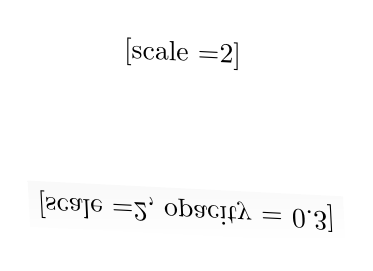
\begin{tikzpicture}
    \node[yslant=-0.05] at (0,0) {\huaslogo[scale =2]};
    \node[yscale=-1,yslant=0.05,xslant=0.05, shade,top color=gray!5, 
        bottom color=white] at (0.05,-2) {\huaslogo[scale =2, 
        opacity = 0.3]};
\end{tikzpicture}}
\end{verbatim}
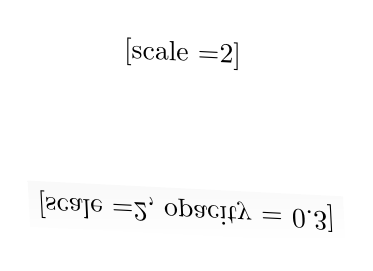
\begin{tikzpicture}
\node[yslant=-0.05] at (0,0) {\huaslogo[scale =2]};
\node[yscale=-1,yslant=0.05,xslant=0.05, shade,top color=gray!5, bottom color=white] at (0.05,-2) {\huaslogo[scale =2, opacity = 0.3]};
\end{tikzpicture}
\begin{verbatim}
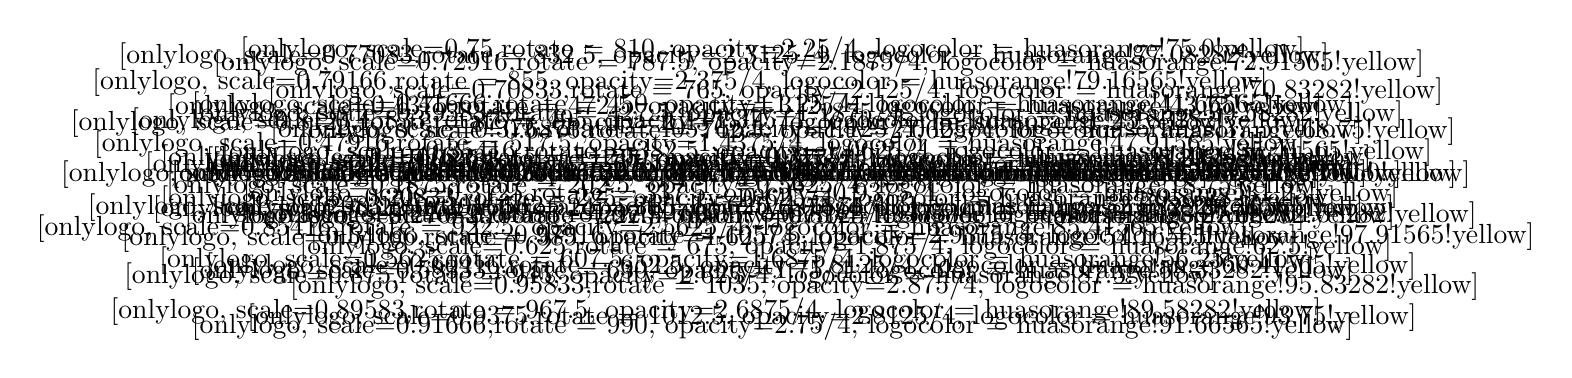
\begin{tikzpicture}
    \node (0,0){} circle (1)
\foreach \ang [evaluate={\j=(\ang / 360)},evaluate={\i=(\ang / 360)/3}, 
    evaluate={\c=(\ang / 1080)*100}] in {0,22.5,...,1080}
    {
    pic at (\ang:\j*0.7 cm) 
        {code={\node {\huaslogo[onlylogo, scale=\i,rotate = \ang, 
        opacity=\j/4, logocolor = huasorange!\c!yellow]};}}
    };
\end{tikzpicture}
\end{verbatim}
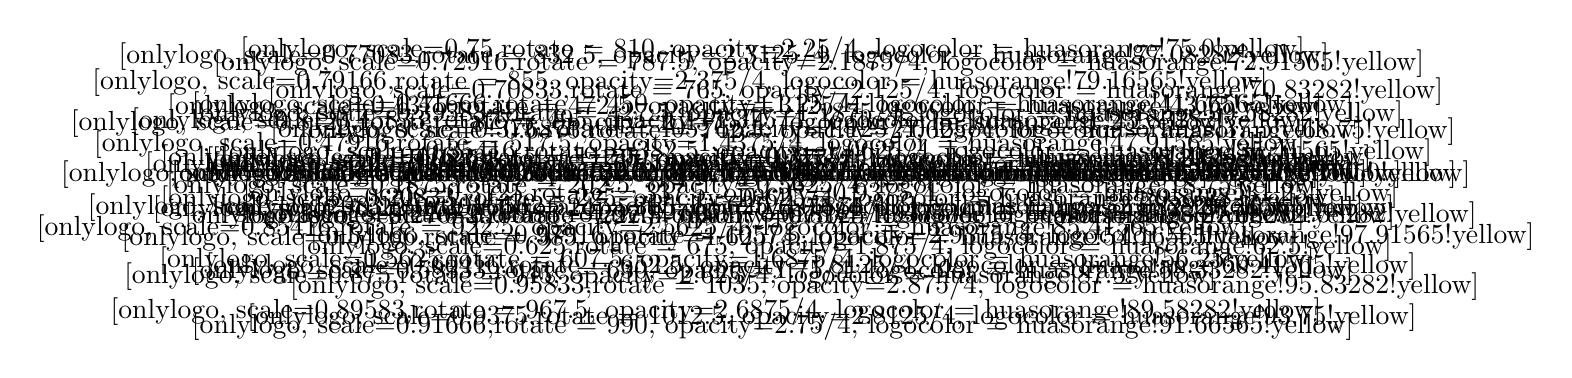
\begin{tikzpicture}
\node (0,0){} circle (1)
\foreach \ang [evaluate={\j=(\ang / 360)},evaluate={\i=(\ang / 360)/3}, evaluate={\c=(\ang / 1080)*100}]  in {0,22.5,...,1080}{
    pic at (\ang:\j*0.7 cm) {code={\node {\huaslogo[onlylogo, scale=\i,rotate = \ang, opacity=\j/4, logocolor = huasorange!\c!yellow]};}}
  };
\end{tikzpicture}
\\
\begin{verbatim}
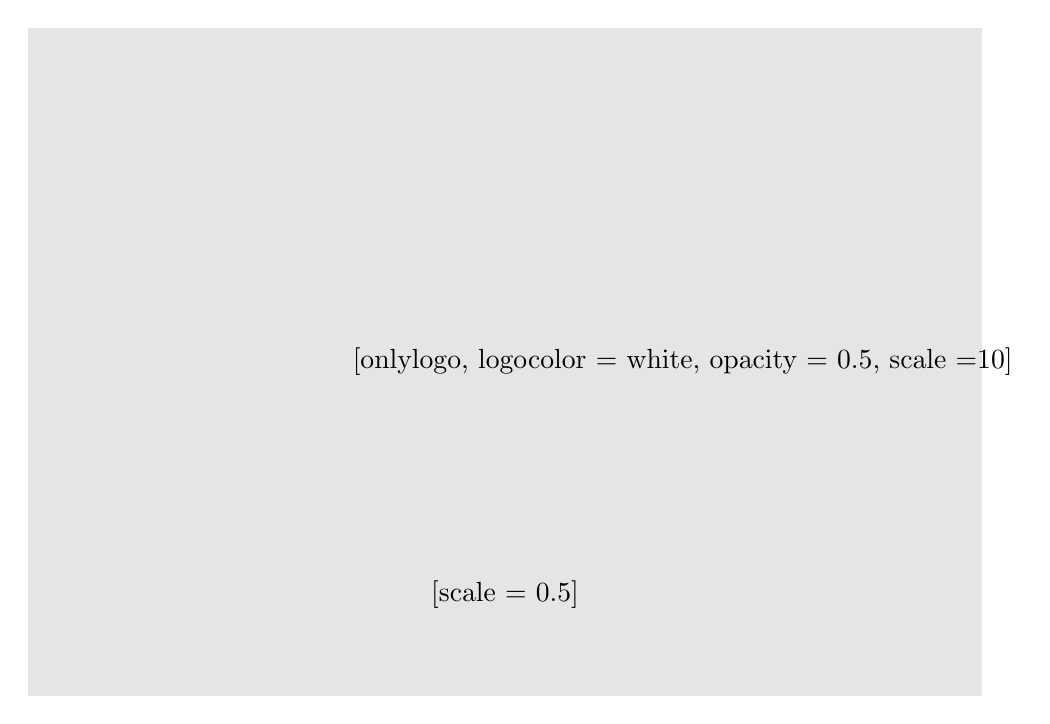
\begin{tikzpicture}
    \node[rectangle, minimum height = 0.7\textwidth,
        minimum width = \textwidth, fill = gray!20](rect) at (0,0){};
    \node[left = -5 mm of rect.east, anchor = east]
        {\huaslogo[onlylogo, logocolor = white, 
            opacity = 0.5, scale =10]};
    \node[below = 0 mm of rect.center, anchor = north]{\huaslogo};
    \node[above = 1 cm of rect.south, anchor = south]
        {\huasSYTMTW[scale = 0.5]};
\end{tikzpicture} 
\end{verbatim}
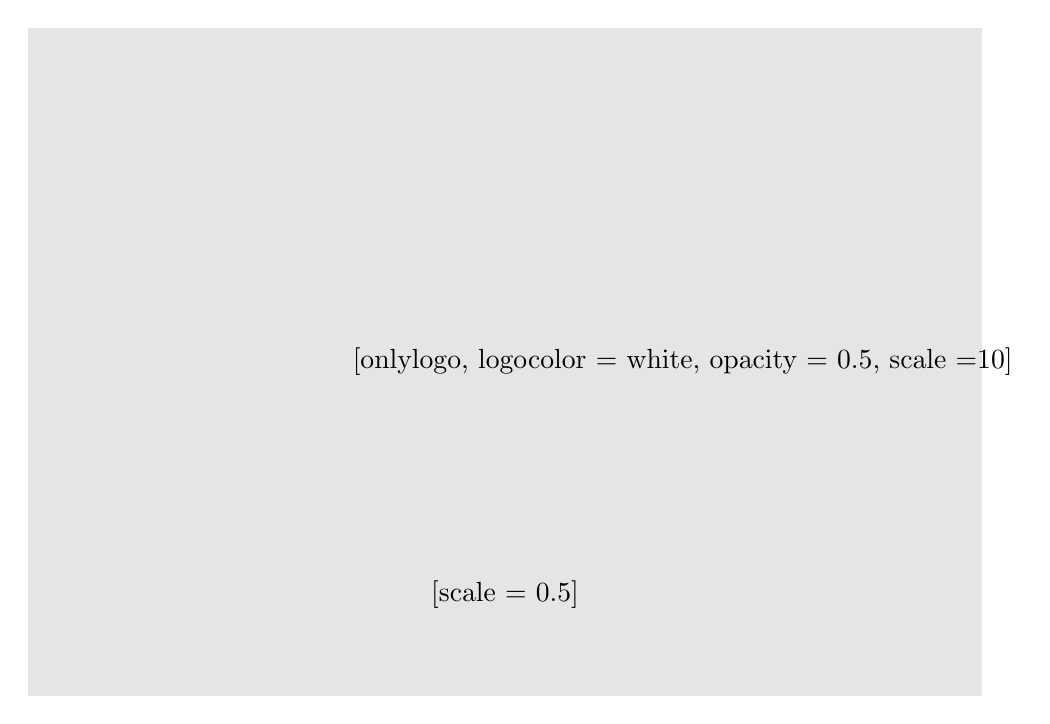
\begin{tikzpicture}
\node[rectangle, minimum height = 0.7\textwidth,minimum width = \textwidth, fill = gray!20](rect) at (0,0){};
\node[left = -5 mm of rect.east, anchor = east]{\huaslogo[onlylogo, logocolor = white, opacity = 0.5, scale =10]};
\node[below = 0 mm of rect.center, anchor = north]{\huaslogo};
\node[above = 1 cm of rect.south, anchor = south]{\huasSYTMTW[scale = 0.5]};

\end{tikzpicture} 
The options for Tikz and the \verb|\huaslogo| can be used in combination.
\par

\section{Changelog}
v1.0 [2023/01/26] Initial release, Logos of HUAS (NL and EN) and SYTMTW. 
\end{document}
